
\subsection{Statement}

This section deals with the steady state version of the problem proposed by Smith and Hutton (1982) described in \cite{smith1982numerical}. The problem takes place in the domain $\Omega = (-L,L) \times (0,L) \subset \real^2$ where $L > 0$ is a constant length. Both density and diffusion coefficient are assumed to be constant and known values. In $\Omega$ the steady state version of the general convection--diffusion equation with no source term is considered, that is,
\begin{equation} \label{eq:smith_hutton_case_pde}
	\frac{\rho}{\Gamma} \vb{v} \vdot \grad{\phi} = \Delta{\phi}
\end{equation}
On the boundary of $\Omega$ the following conditions are prescribed:
\begin{itemize}[topsep=0pt]
	\item $\phi = 1 + \tanh(10(2x+1))$ on $C_1 = [-L,0] \times \{ 0 \}$ (inlet flow).
	\item $\phi = 1 - \tanh(10)$ on $C_2 = \left( \{ -L \} \times (0,L) \right) \cup \left( [-L,L] \times \{ L \} \right) \cup \left( \{ L \} \times [0,L) \right)$.
	\item $\dfrac{\partial \phi}{\partial y} = 0$ on $C_3 = (0,L) \times \{ 0 \}$ (outlet flow).
\end{itemize}
Notice that the curves $C_1, C_2, C_3$ give a partition of $\partial \Omega$. To encode the first two boundary conditions in a compact manner, we define the function $g \colon C_1 \cup C_2 \rightarrow \real$ by
\begin{equation}
	g(x,y) = 
	\left\{
	\begin{aligned}
		&1 + \tanh(10(2x + 1)) 	& &\text{if } (x,y) \in C_1 \\
		&1 - \tanh(10) 			& &\text{if } (x,y) \in C_2
	\end{aligned}
	\right.
\end{equation}
The velocity field is given by $u = 2 y (1 - x^2)$ and $v = -2 x (1 - y^2)$. The Cauchy problem resulting from the PDE \eqref{eq:smith_hutton_case_pde} and the boundary conditions is given by \eqref{eq:smith_hutton_cauchy_problem} and is summarized in figure \ref{fig:smith_hutton_cauchy_problem}.
\begin{equation} \label{eq:smith_hutton_cauchy_problem} 
	\left\{
	\begin{aligned}
		&\Delta \phi - \frac{\rho}{\Gamma} \vb{v} \vdot \grad{\phi} = 0 &
		&\text{in } \Omega \\
		&\phi = g & 
		&\text{on } C_1 \cup C_2 \\
		&\frac{\partial \phi}{\partial y} = 0 & 
		&\text{on } C_3
	\end{aligned}
	\right.
\end{equation}

\begin{figure}[h]
	\centering
	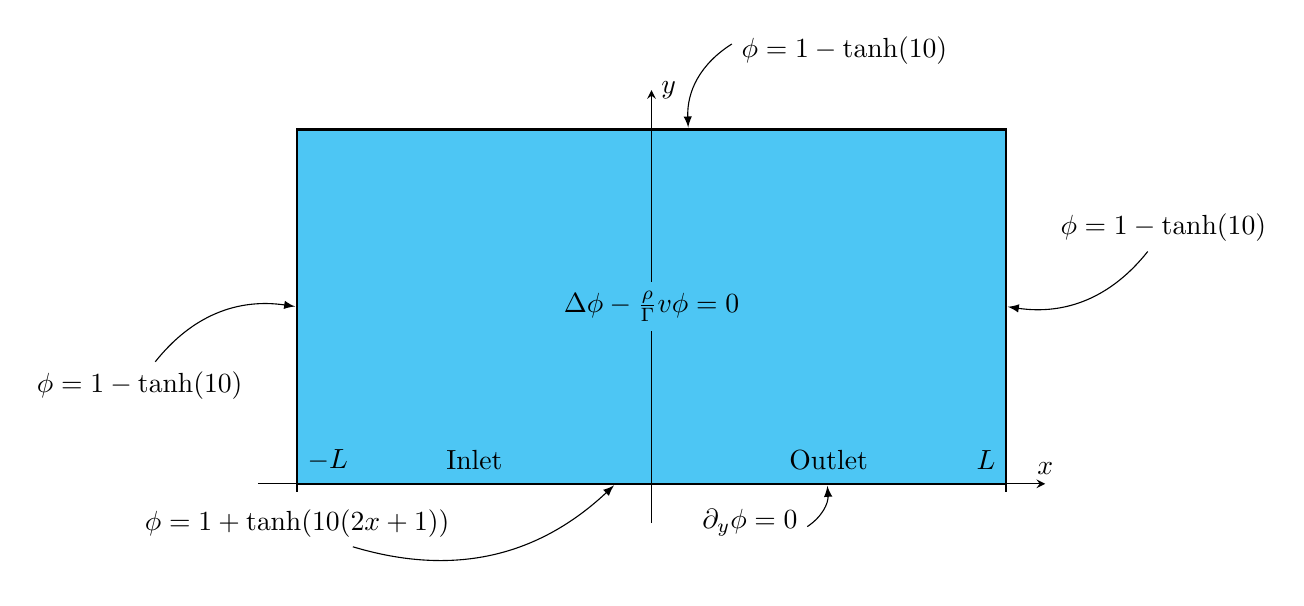
\begin{tikzpicture}
		% Lenghts
		\def\alength{5}
		\def\L{4.5}
		\def\mlength{0.1}
		% Domain
		\fill[cyan!70!white] (-\L,0) rectangle (\L, \L);
		\draw[thick, thick] (-\L,0) rectangle (\L, \L);
		% Axis
		\draw[-stealth] (-\alength,0) -- (\alength,0) node[above]{$x$};
		\draw[-stealth] (0,-0.5) -- (0,\alength) node[right]{$y$};
		\draw[black, thick] (\L,0) node[left, yshift=3mm]{$L$} -- ++(0,-\mlength);
		\draw[black, thick] (-\L,0) node[right, yshift=3mm]{$-L$} -- ++(0,-\mlength);
		% Right boundary condition
		\node[inner sep=0pt] at (\L,{0.5*\L}) (rb) {};
		\node[] at ({\L+2},{0.5*\L+1}) (rbc) {$\phi = 1 - \tanh(10)$};
		\path[-latex] (rbc) edge[bend left] node [left] {} (rb);
		% Top boundary condition
		\node[inner sep=0pt] at ({0.1*\L},\L) (tb) {};
		\node[] at ({0.1*\L+2},{\L+1}) (tbc) {$\phi = 1 - \tanh(10)$};
		\path[-latex] (tbc) edge[bend right] node [left] {} (tb);
		% Left boundary condition
		\node[inner sep=0pt] at (-\L,{0.5*\L}) (lb) {};
		\node[] at (-\L-2,{0.5*\L-1}) (lbc) {$\phi = 1 - \tanh(10)$};
		\path[-latex] (lbc) edge[bend left] node [left] {} (lb);
		% Right bottom boundary condition
		\node[inner sep=0pt] at ({0.5*\L},0) (bb) {};
		\node[] at ({0.5*\L-1},-0.5) (bbc) {$\partial_y \phi = 0$};
		\path[-latex] (bbc) edge[bend right] node [left] {} (bb);
		% Left bottom boundary condition
		\node[inner sep=0pt] at ({-0.1*\L},0) (lbb) {};
		\node[] at ({-\L},-0.5) (lbbc) {$\phi = 1 + \tanh(10(2x+1))$};
		\path[-latex] (lbbc) edge[bend right] node [left] {} (lbb);
		% PDE outer sep=0pt, greenNode, yshift=3mm, fill=white
		\node[fill=cyan!70!white] at (0,{0.5*\L}) 
		{$\Delta \phi - \frac{\rho}{\Gamma} \vb{v} \vdot \grad{\phi} = 0$};
		% Inlet and outlet
		\node[] at ({-0.5*\L},0.3) {Inlet};
		\node[] at ({0.5*\L},0.3) {Outlet};
	\end{tikzpicture}
	\caption{Cauchy problem for the diagonal flow case.}
	\label{fig:smith_hutton_cauchy_problem}
\end{figure}





